\documentclass[12pt]{article}

\usepackage{amsmath,amsfonts,stmaryrd,amssymb} % Math packages
\usepackage{enumerate} % Custom item numbers for enumerations
\usepackage[ruled]{algorithm2e} % Algorithms
\usepackage[framemethod=tikz]{mdframed} % Allows defining custom boxed/framed environments
\usepackage{listings} % File listings, with syntax highlighting
\lstset{
	basicstyle=\ttfamily, % Typeset listings in monospace font
}


%Fonts
\usepackage[utf8]{inputenc} % Required for inputting international characters
\usepackage[T1]{fontenc} % Output font encoding for international characters
\usepackage{XCharter} % Use the XCharter fonts

% For using Subfigures
\usepackage{caption}
\usepackage{subcaption}
%	DOCUMENT MARGINS
\usepackage{geometry} % Required for adjusting page dimensions and margins
\usepackage{graphicx,wrapfig,lipsum}
\usepackage{hyperref}

\geometry{
	paper=a4paper, % Paper size, change to letterpaper for US letter size
	top=2.5cm, % Top margin
	bottom=3cm, % Bottom margin
	left=2.5cm, % Left margin
	right=2.5cm, % Right margin
	headheight=14pt, % Header height
	footskip=1.5cm, % Space from the bottom margin to the baseline of the footer
	headsep=1.2cm, % Space from the top margin to the baseline of the header
	%showframe, % Uncomment to show how the type block is set on the page
}
%----------------------------------------------------------------------------------------
%	INFORMATION ENVIRONMENT
%----------------------------------------------------------------------------------------

% Usage:
% \begin{info}[optional title, defaults to "Info:"]
% 	contents
% 	\end{info}

\mdfdefinestyle{info}{%
	topline=false, bottomline=false,
	leftline=false, rightline=false,
	nobreak,
	singleextra={%
		\fill[black](P-|O)circle[radius=0.4em];
		\node at(P-|O){\color{white}\scriptsize\bf i};
		\draw[very thick](P-|O)++(0,-0.8em)--(O);%--(O-|P);
	}
}

% Define a custom environment for information
\newenvironment{info}[1][Info:]{ % Set the default title to "Info:"
	\medskip
	\begin{mdframed}[style=info]
		\noindent{\textbf{#1}}
	}{
	\end{mdframed}
}
% ----------------------------------------------------------

%----------------------------------------------------------------------------------------

%\setcounter{secnumdepth}{0} % For removing numbers from the section
\setlength{\parindent}{0em} % Setting Paragraph indent for the document to 0.
%Scribing Start from here
%Body
\begin{document}
	\newgeometry{top=5cm,bottom=0.1cm}
	\begin{titlepage}
		\begin{center}
			\textbf{\LARGE \vspace*{15pt}Indian Institute of Technology, Kanpur}
		\end{center}
		\begin{figure}[h]
			\centering
			
\includegraphics[scale=0.7]{images/bluelog.jpg}
		\end{figure}
		\vspace{1cm}
		\begin{center}
			\textbf{\LARGE CS685A: Data Mining}
			
			\bigskip
			\textbf{\LARGE Assignment 2\\}
		\end{center}
		
		
		\begin{center}
			\vspace{1 cm}
			\Large
			\textbf{Supervised by: Dr. Arnab Bhattacharya}\\
			\vspace{30pt}
			November 16,2020
		\end{center}
		
		
		\bigskip
		\vspace{1cm}
		\centering
		\large
		Submitted By:
		Aditya Jain\\
		20111004\\
		\texttt{adityaj20@iitk.ac.in}\\
		
		
		
	\end{titlepage}
	\newpage
	
	\restoregeometry
	\renewcommand*\contentsname{\centering Table of Contents \bigskip}
	\tableofcontents
	
	%----------------------------------------------------------------------------------------
	%	INTRODUCTION
	%----------------------------------------------------------------------------------------
	\newpage
	\section{Introduction} % Unnumbered section
	
	I have done analysis on the dataset that contains the human navigation paths on Wikipedia, collected through the human-computation game "Wikispeedia". Wikispeedia, users are asked to navigate from a given source to a given target article, by only clicking Wikipedia links. A condensed version of Wikipedia (4,604 articles) is used.  
	
	\subsection{Data collection}
	
	Data for this study is collected from \url{http://snap.stanford.edu/data/wikispeedia.html}. Following tsv files are incorporated for data processing to generate the results. These are available in wikispeedia paths-and-graph.tar.gz. 
	\begin{enumerate}
	    \item articles.tsv
	    \item categories.tsv
	    \item paths\_finished.tsv
	    \item paths\_unfinished.tsv
	    \item shortest-path-distance-matrix.txt
	\end{enumerate}
	
	\subsection{Data Correction and Pre-processing}
	Following changes are made inside the programs to correct the errors in the file.
	\begin{itemize}
		\item There exists 6 articles for which no category is defined in category.tsv, so I have assigned them to category "subject". (Q3)
		\item Paths of length zero are removed from paths\_finished.tsv as they are invalid for the scenario. (Q6)
	    \item Due to errors in article names in  paths\_unfinished.tsv, I have renamed the article names for which a possible valid article name was present and others are assigned to category subject as no suitable mapping exists for them. (Q10)
	    
	  
	\end{itemize}
	
	A total of 4,604 articles exist in our experiment and these articles belongs to 146 different categories. There are 51,306 valid finished paths and 24,875 valid unfinished paths in the analysis domain dataset.
	
	\pagebreak
	\section{Observations \& Analysis} % Numbered section
	
	\subsection{Wikipedia Articles and Categories}
	We are analyzing a total of 4604 Wikipedia Articles. These articles are assigned to 146 different categories. These categories are sub-categorized level wise:
	\begin{table}[h]
	\centering
	\begin{tabular}{|l|l|}
	\hline
	Number of Categories at level 1 & 1   \\ \hline
	Number of Categories at level 2 & 15  \\ \hline
	Number of Categories at level 3 & 130 \\ \hline
	\end{tabular}
	\caption{Number of sub-categories at each level}
	\end{table}
	
	After assigning categories to each article, I found that there are 6 such articles which do not belong to any category. So to use these articles in the analysis, "subject" category is assigned to these 6 categories. Table 2 shows that there are only 8 articles that belongs to exactly 3 categories. So we can infer that our sample size include articles which are restricted to few categories only.
	\begin{table}[h]
	\centering
	\begin{tabular}{|l|l|}
	\hline
	Articles belonging to at least 1 category     & 4598 \\ \hline
	Articles belonging to at least 2 categories   & 598  \\ \hline
	Articles belonging to at exactly 3 categories & 8    \\ \hline
	\end{tabular}
	\caption{Number of categories to which an article belongs to}
	\end{table}
	
	%------------------------------------------------
	\subsection{Connectivity of articles in Wikipedia}
	\begin{table}[h]
	\centering
	\begin{tabular}{|l|l|l|}
	\hline
	Nodes & Edges  & Diameter \\ \hline
	4589  & 106534 & 5        \\ \hline
	3     & 3      & 1        \\ \hline
	1     & 0      & 0        \\ \hline
	1     & 0      & 0        \\ \hline
	1     & 0      & 0        \\ \hline
	1     & 0      & 0        \\ \hline
	1     & 0      & 0        \\ \hline
	1     & 0      & 0        \\ \hline
	1     & 0      & 0        \\ \hline
	1     & 0      & 0        \\ \hline
	1     & 0      & 0        \\ \hline
	1     & 0      & 0        \\ \hline
	1     & 0      & 0        \\ \hline
	1     & 0      & 0        \\ \hline
	\end{tabular}
	\caption{Connected components of graph made on articles}
	\end{table}
	In our sample size of 4604 articles, we found that there are 14 connected components in which the largest component has 4589 articles. This shows that the articles are very well connected to each other. The diameter of the graph drawn of these 4589 connected articles is 5, which means that an user will require to click on at most 5 links to go from any article to any other article among these 4589 articles.\\
	
	There are 12 isoloated articles which are not connected to any other article. So if user lands to any of these articles it cannot go to any other article through the wikipedia's web interface. He/She needs to go back to search engine to go to another article. 
	
	\subsection{Reachability of articles in Wikipedia}
	In the game, user is asked to go from one source article to a destination article through the interface of Wikipedia by clicking on the links present on the articles. Path that user followed to reach the destination is referred as "Human Path" in the entire report.\\
	
	Figure 1 is a Pi chart which shows the comparision of human path lengths and their corresponding shortest path length in terms of percentage. This results are made from 51,306 test cases.
\begin{figure}[h]
    \centering
    \hspace{-60pt}
    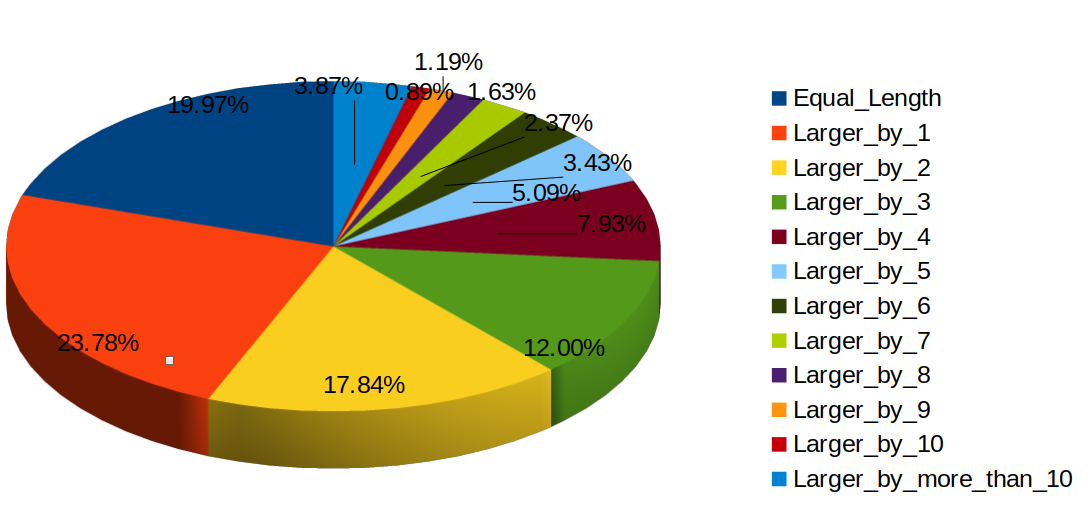
\includegraphics[scale = 0.47]{images/percentage_pi.png}
    \caption{Comparision of Human path to its corresponding shortest path length}
\end{figure}
\pagebreak

\begin{figure}[h]
    \centering
    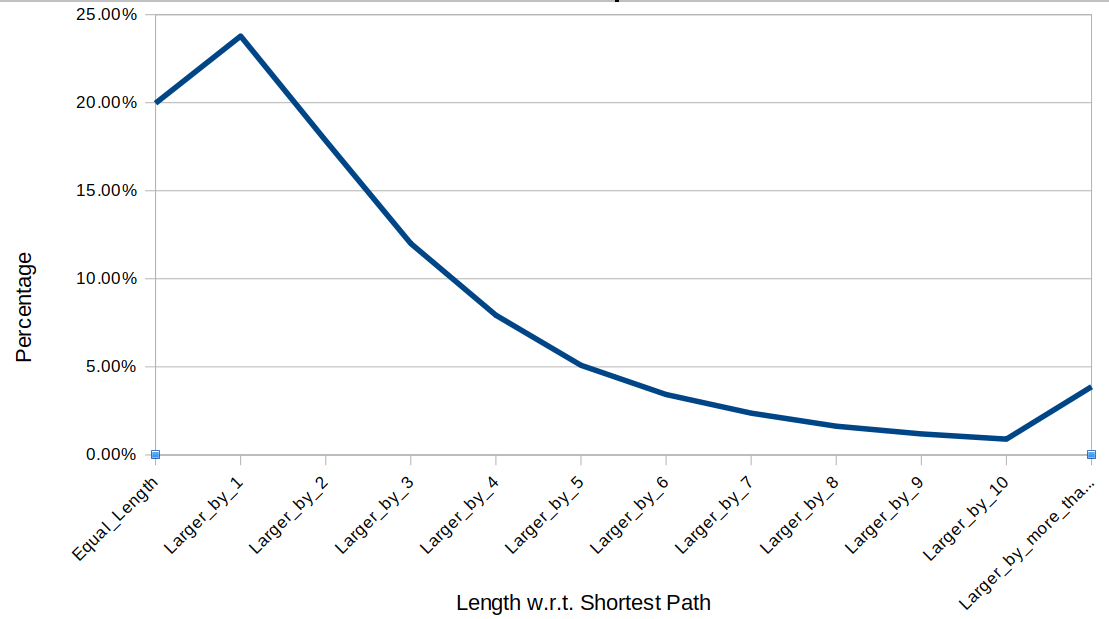
\includegraphics[scale = 0.3]{images/percentage_path_line.png}
    \caption{}
\end{figure}

In Figure 2, we can see that around 20\% of human paths are equal to their corresponding shortest path. There are 23.78\% paths for which human path length is one more than its corresponding shortest length. This shows that Wikipedia article interface is quite readable and interpretable that users are able to move accross the articles very easily. 

\subsubsection{With Backlinks}
There is a exponential fall in the percentage as we move accross the x-axis and increase the human path length. 

Since around 60\% of test cases have reasonable human path length, we can conclude that Wikipedia pages are quite reachable and user-friendly. 

\subsubsection{Without Backlinks}
\begin{figure}[h]
    \centering
    \hspace{-60pt}
    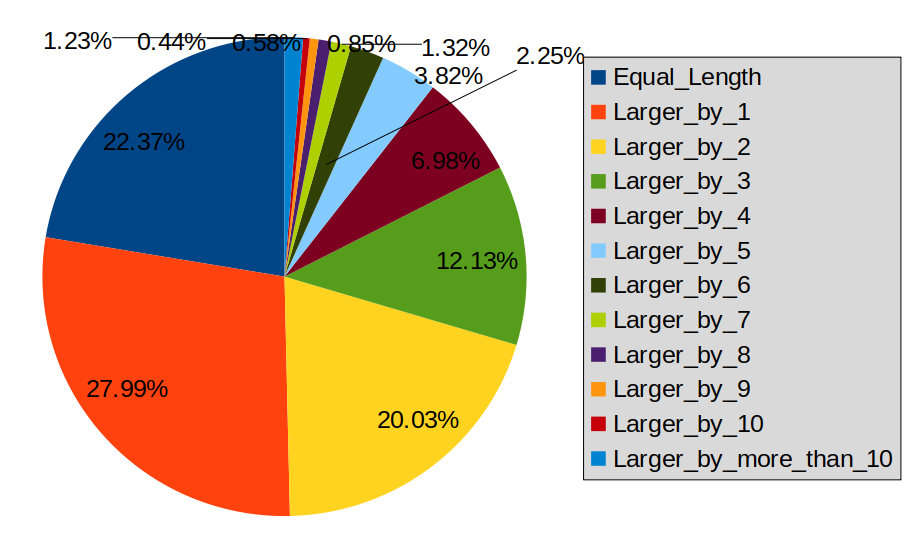
\includegraphics[scale = 0.4]{images/percentage_pi_noback.png}
    \caption{Comparision of Human path to its corresponding shortest path length}
\end{figure}

\begin{figure}[h]
    \centering
    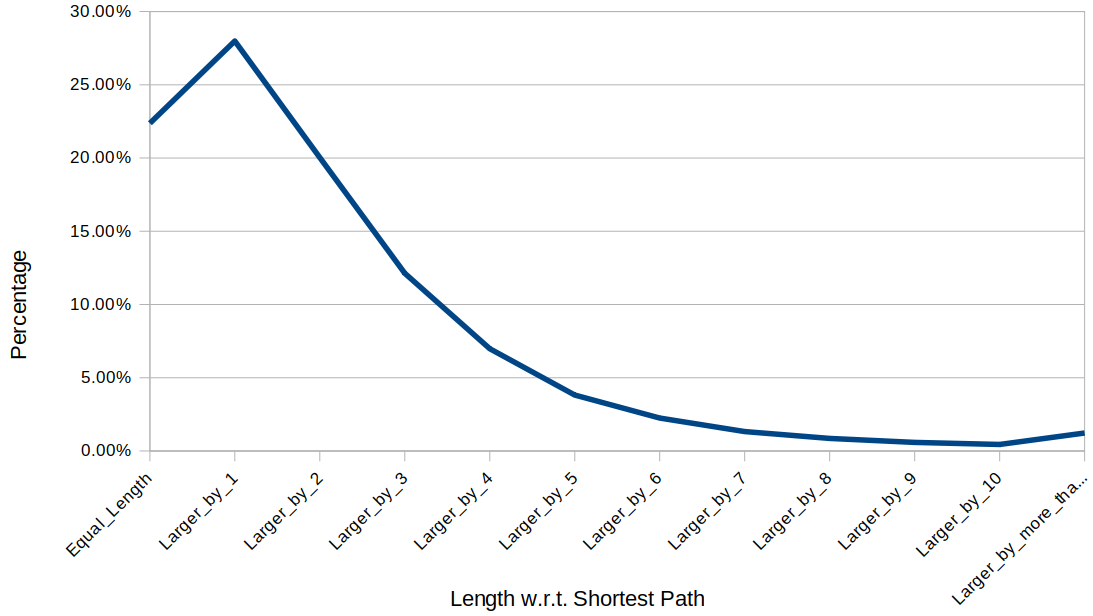
\includegraphics[scale = 0.28]{images/percentage_noback_line.png}
    \caption{}
\end{figure}
Back clicks: User clicking on the back button on the brower to go back to the last article.
Here we have ignore the back clicks made by the user and we found that now 70\% of the test cases are of reasonable length. There is an increase of 10\%. Since this increase of 10\% is occuring in the human path length greater than one, this shows that user is able to identify that he/she has traversed to a wrong article just after going to that wrong article. So we can concur that Wikipedia articles are quite interpretable that user is able to identify his/her mistake.


\subsection{Category Analysis}	

\subsubsection{Popularity of Categories}
\subsubsection{Bottom-Up Analysis}
\begin{figure}[h]
    \centering
    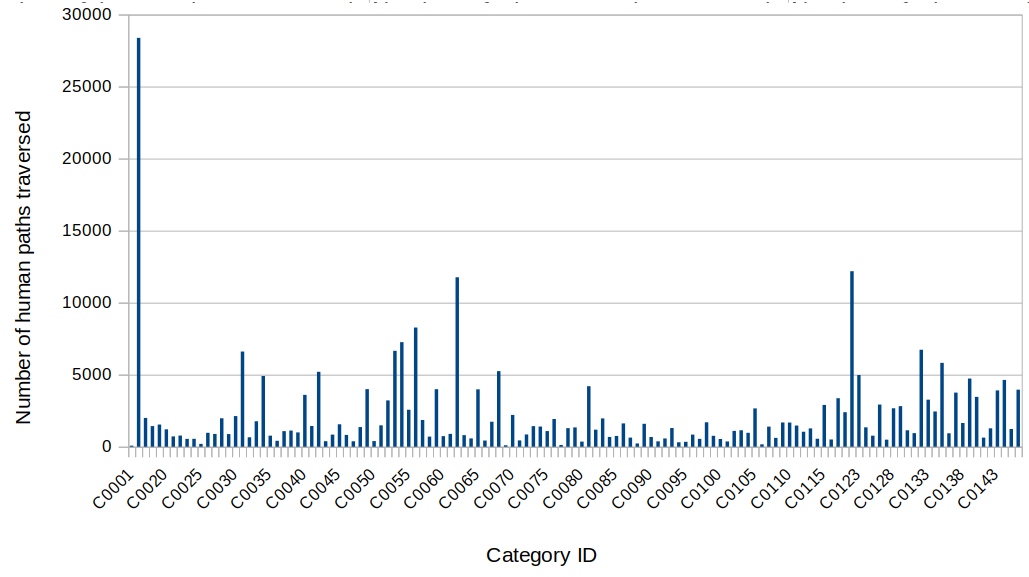
\includegraphics[scale = 0.4]{images/q8_number_of_paths.png}
    \caption{Bottom-Level Category ID vs Number of Human Paths they occur}
\end{figure}
\pagebreak

\begin{figure}[h]
    \centering
    \hspace{-60pt}
    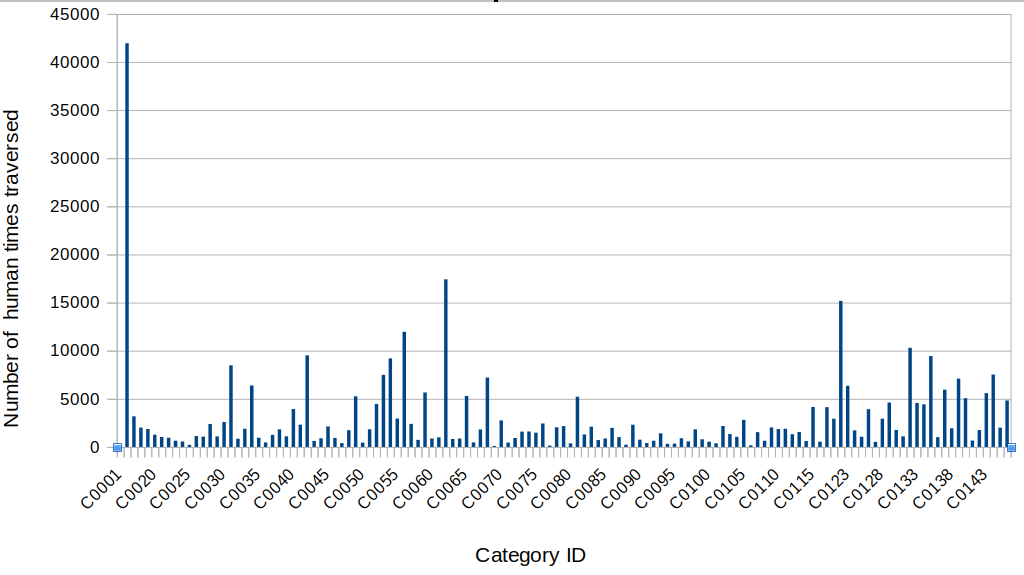
\includegraphics[scale = 0.47]{images/q8_number_of_times.png}
    \caption{Category ID vs Number of times they occur in Human Paths}
\end{figure}

Figure 5 shows the number of paths in which a category is occured whereas Figure 6 shows the number of times a category is occured in the whole test case. Both are the results for the category at bottom most level, here we are focusing on the broadest granularity. So out of these 130 categories top 10 most popular categories are : 
\begin{table}[h]
\centering
\begin{tabular}{|l|}
\hline
Category ID \\ \hline
C0005       \\
C0122       \\
C0062       \\
C0056       \\
C0054       \\
C0132       \\
C0053       \\
C0031       \\
C0135       \\
C0068      	\\ \hline	
\end{tabular}
\caption{Top 10 Popular Categories}
\end{table}

These are the categories which occured in most of the human paths. Category C0005 occured in 28,375 times alone. 
\pagebreak

\subsubsection{Top-Down (Sub-Categories) Analysis}
\begin{figure}[h]
    \centering
    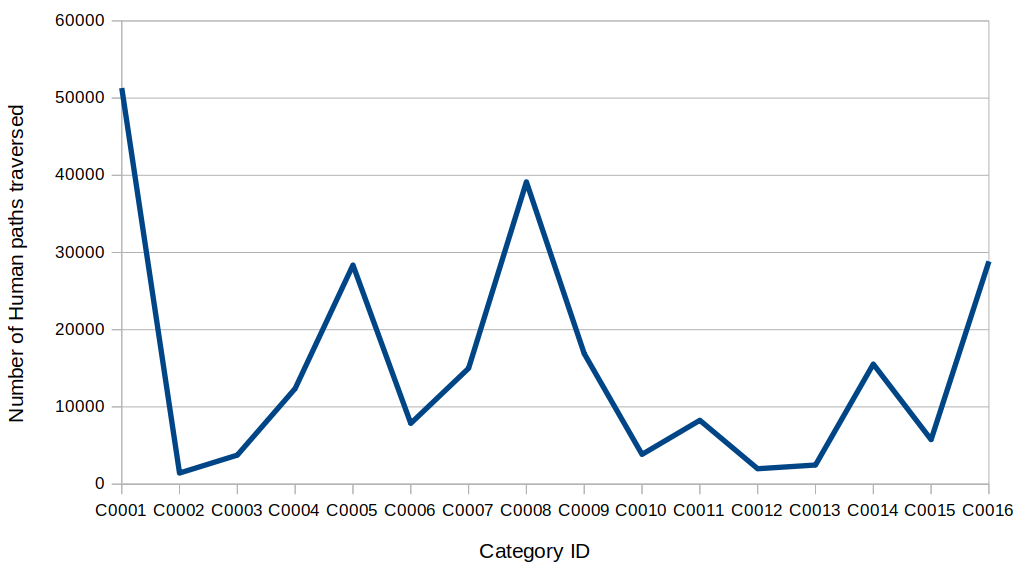
\includegraphics[scale = 0.47]{images/q9_paths.png}
    \caption{Top-level Category ID vs Number of Human Paths they occur}
\end{figure}
 Here focus on 16 categories at level 1 and 2. These are parent to the 130 categories categories at level 3. Figure 7 shows the number of human paths in which these categories have occured. Top 5 popular categories are:
\begin{table}[h]
\centering
\begin{tabular}{|l|}
\hline
Category\_ID \\ \hline
C0001        \\
C0008        \\
C0016        \\
C0005        \\
C0117        \\ \hline
\end{tabular}
\caption{Top 5 populuar categories}
\end{table}
Since C0001 is parent to all the categories, it is obvious for it to occur on top. After it C008, C0016 and C0005 are the most popular categories that are occuring in the search pattern of the users.
\pagebreak

\subsection{Shortest Path Analysis}
For each source and destination article pair that user was asked to traverse, we found the shortest path of articles. Following is an analysis on the categories that occured in the shortest path corresponding to each test case.
\begin{figure}[h]
    \centering
    \hspace{-60pt}
    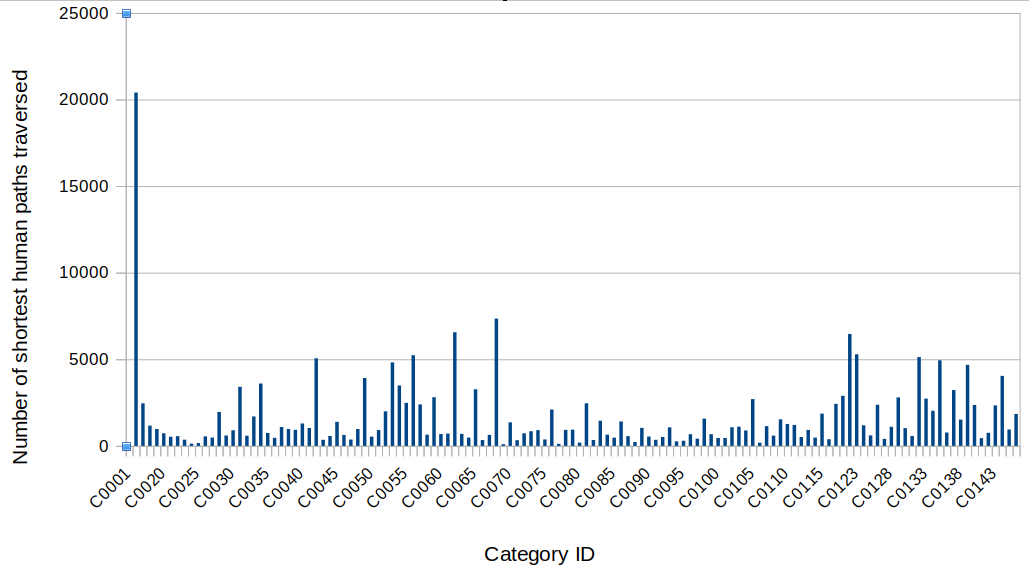
\includegraphics[scale = 0.47]{images/q8_number_of_shortest_paths.png}
    \caption{Category ID vs Number of times they occur in shortest path}
\end{figure}

Figure 8 shows the categories that occur in the shortest path for each test case of source and destination article. From the above graph we can tell the categories which are not only most popular but are also most reachable. These categories come in the shortest paths shows that they are very much related to other categories.\\

\begin{figure}[h]
    \centering
    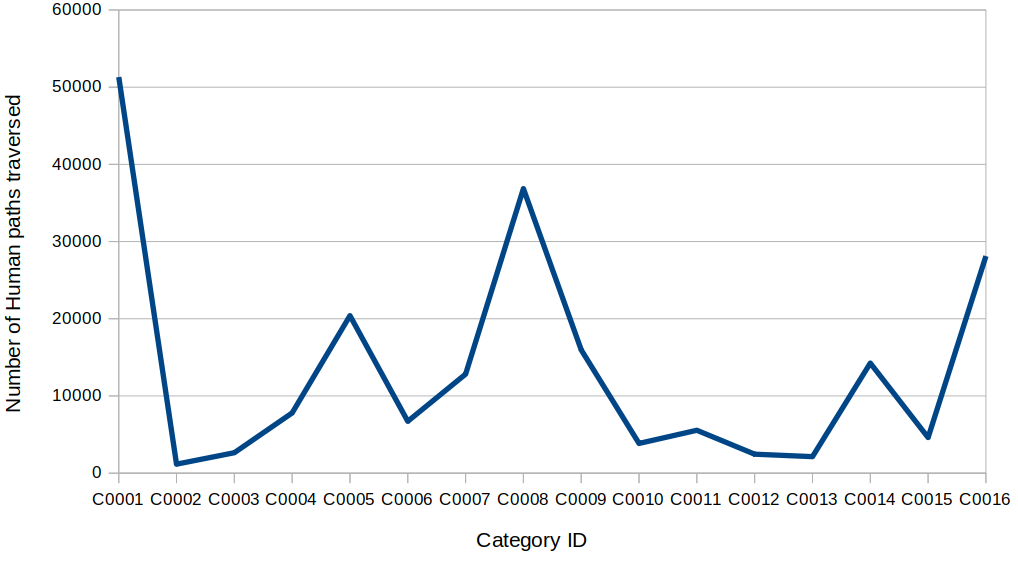
\includegraphics[scale = 0.33]{images/q9_shortest_paths.png}
    \caption{Top-level Category ID vs Number of shortest paths they occur}
\end{figure}

Figure 9 shows the categories that occur in the shortest path for each test case but here we only considered the categories at level 1 and 2.\\
Category IDs C0005, C0068, C0062, C0122, and C0123 occured most times in bottom-up analysis, whereas C0001, C0008, C0016, C0005, and C0117 occured most times in top-down analysis. This shows that these categories are most similar to other categories. 


\subsection{Category-Pair Analysis}
Observation and results are as follows:
\begin{itemize}
	\item Total of 17,196 category pairs exists for complete test case.
	\item Total of 15,356 category pairs exist for the finished paths.
	\item Total of 13,754 category pairs exist for the unfinished paths.
	\item There are 1,840 category pairs which are not connected, i.e. user can't traverse from one category to another through links.
	\item There are 1,419 category pairs have equal probablity to be completed by the user or left by the user in middle.
	\item There are 1,648 category pairs for which no finished test case exist, suggesting that these category pairs are unreachable. 
\end{itemize}

\begin{figure}[h]
    \centering
    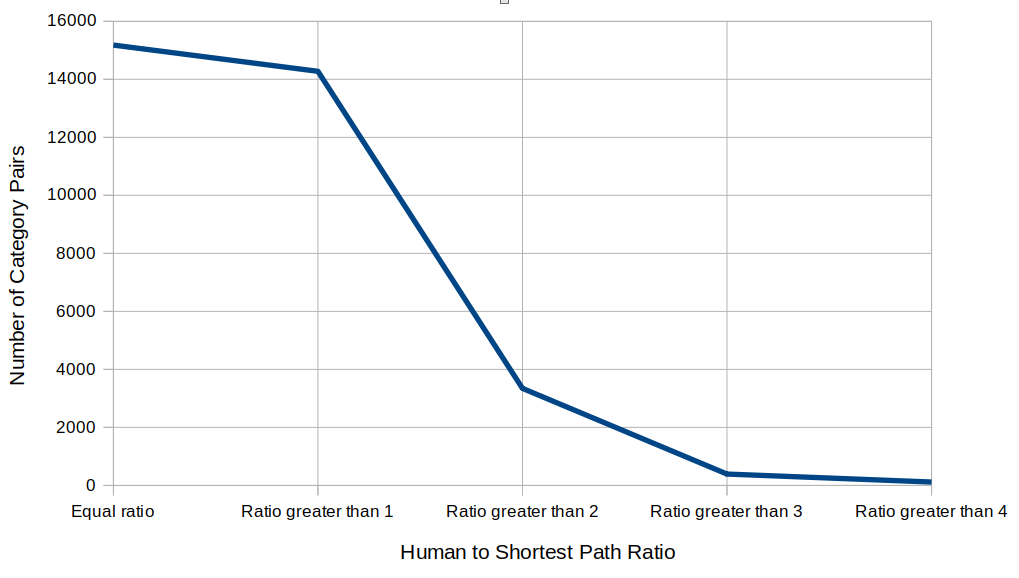
\includegraphics[scale = 0.33]{images/q11.png}
    \caption{Number of category pairs in a Human/Shortest path ratio segment}
\end{figure}

Results from Figure 10:
\begin{itemize}
	\item There are 1,081 category pairs whose ratio is 1.
	\item There are 14,275 category pairs whose ratio is more than 1.
	\item Ther are only 3,345 category pairs whose ratio is more than 2.
	\item Only 391 category pairs whose ratio is more than 3. 
	\item Only 117 whose ratio is equal or more than 4.
\end{itemize}

There are 94.04\% category pairs whose human to shortest path length is less than 2. This shows that Wikipedia's interface is very user-friendly such that user can traverse from one category's article to another category's article without any hassle.
	
\section{Conclusion}
\begin{itemize}
	\item The articles are very well connected to each other. The user will require to click on at most 5 links to go from any article to any other article among most of the articles. Maximum path size is 9 links, but there are very few such cases.
	\item Wikipedia article interface is quite readable and interpretable that users are able to move accross the articles very easily using forward and backward links.
	\item There are 94.04\% category pairs whose human to shortest path length is less than 2. This shows that Wikipedia's interface is very user-friendly such that user can traverse from one category's article to another category's article without any hassle.
\end{itemize}









  





	
\end{document}